\newcommand{\rover} {rover3/roverLinear1d3}
\newcommand{\pir} {pir/piramid2d}

Rover:
\begin{figure}[h]
\center
\fbox{\includegraphics[scale=0.8]{Figures/\rover-Nodes.eps} }
\caption{An approximation reducing the number of cases.}
\label{steplin} 
\end{figure}

\begin{figure}[h]
\center
\fbox{\includegraphics[scale=0.8]{Figures/\rover-TotTime.eps} }
\caption{An approximation reducing the number of cases.}
\label{steplin} 
\end{figure}

\begin{figure}[h]
\center
\fbox{\includegraphics[scale=0.8]{Figures/\pir-Nodes.eps} }
\caption{An approximation reducing the number of cases.}
\label{steplin} 
\end{figure}

\begin{figure}[h]
\center
\fbox{\includegraphics[scale=0.8]{Figures/\pir-TotTime.eps} }
\caption{An approximation reducing the number of cases.}
\label{steplin} 
\end{figure}

\begin{figure}[h]
\center
\fbox{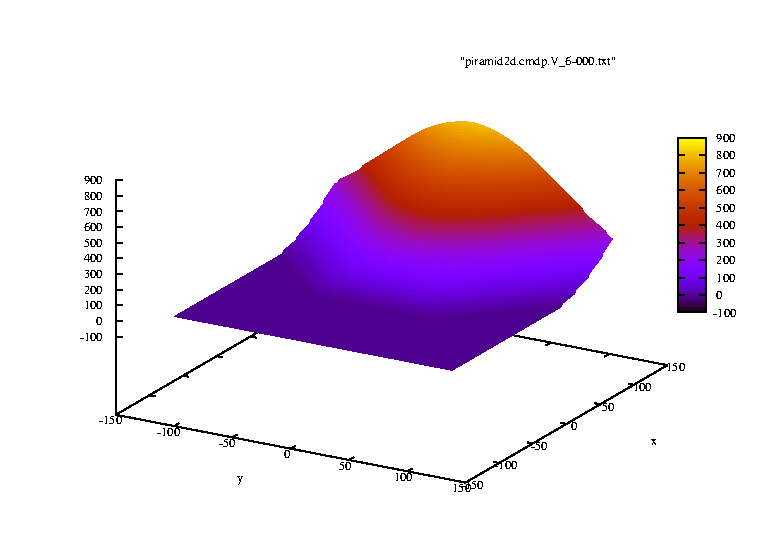
\includegraphics[scale=0.8]{Figures/piramidV6-0.eps} }
\caption{An approximation reducing the number of cases.}
\label{steplin} 
\end{figure}

\begin{figure}[h]
\center
\fbox{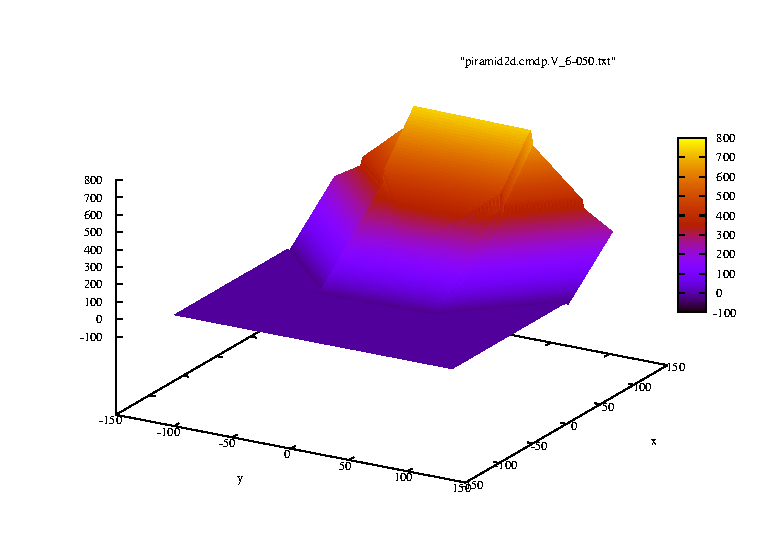
\includegraphics[scale=0.8]{Figures/piramidV6-5.eps} }
\caption{An approximation reducing the number of cases.}
\label{steplin} 
\end{figure}

\begin{figure}[h]
\center
\fbox{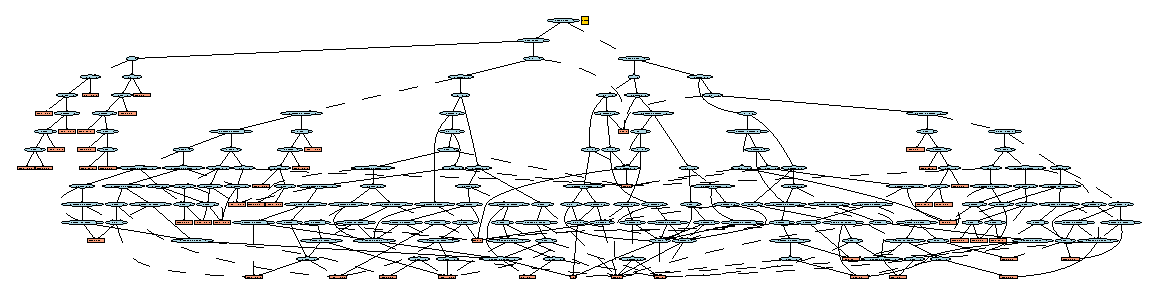
\includegraphics[scale=0.8]{Figures/pirV6-0xadd.eps} }
\caption{An approximation reducing the number of cases.}
\label{steplin} 
\end{figure}

\begin{figure}[h]
\center
\fbox{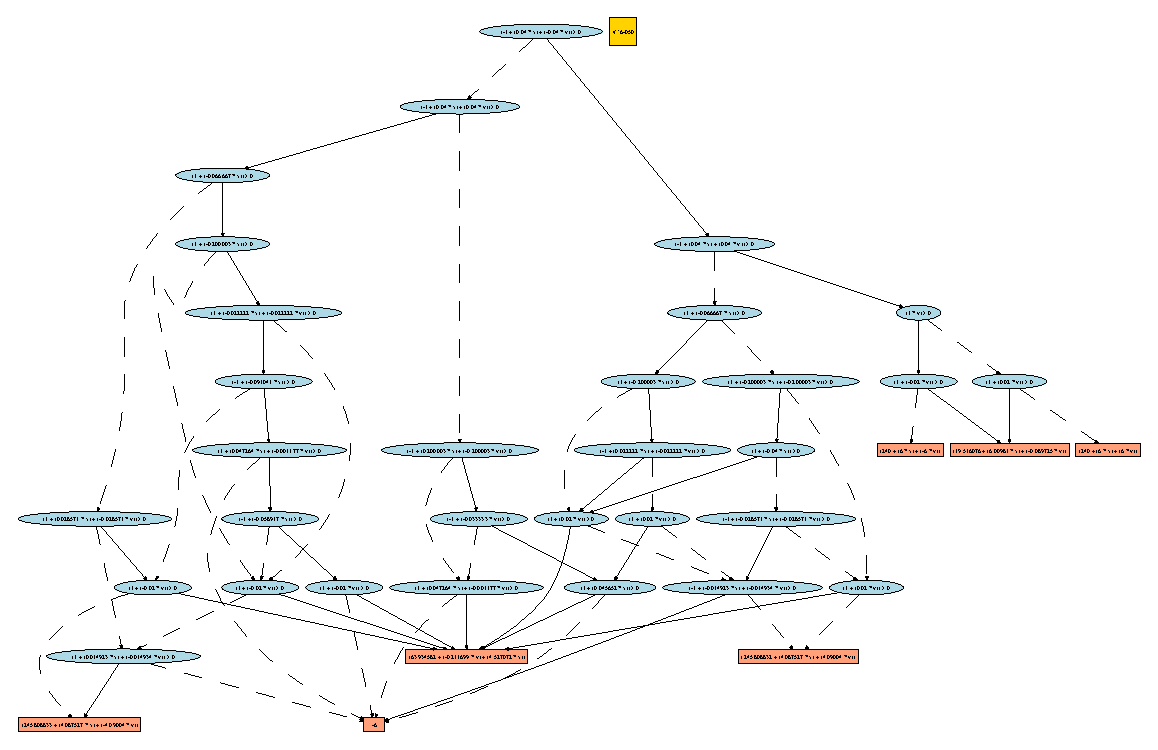
\includegraphics[scale=0.8]{Figures/pirV6-5xadd.eps} }
\caption{An approximation reducing the number of cases.}
\label{steplin} 
\end{figure}